% =====================================================================
% main.tex: root file. Compile this file (pdfLaTeX + BibTeX).
% It holds no report text: it loads the preamble, sets the metadata,
% and pulls in the sections in order.
% =====================================================================
\documentclass[12pt,a4paper]{article}
% =====================================================================
% preamble.tex: packages and project-wide macros. Loaded by main.tex.
% =====================================================================

% Encoding, fonts, language
\usepackage[T1]{fontenc}
\IfFileExists{lmodern.sty}{\usepackage{lmodern}}{} % Latin Modern (present on Overleaf)
\usepackage[american]{babel}
\usepackage{microtype}

% Page layout
\usepackage[a4paper,margin=2.5cm,headheight=15pt]{geometry}
\usepackage{setspace}
\setstretch{1.1}
\usepackage{fancyhdr}
\pagestyle{fancy}
\fancyhf{}
\fancyfoot[C]{\thepage}
\renewcommand{\headrulewidth}{0.4pt}

% Mathematics and numbers
\usepackage{amsmath}
\usepackage{siunitx}
\sisetup{group-separator={,}, group-minimum-digits=4} % \num{10863} prints 10,863

% Tables
\usepackage{booktabs}        % \toprule, \midrule, \bottomrule
\usepackage{array}
\usepackage{threeparttable}  % notes below a table

% Figures
\usepackage{graphicx}
\usepackage{placeins} % \FloatBarrier: keeps floats inside their part of the document
\usepackage{float}    % [H]: places a table exactly where it stands in the source
\graphicspath{{figures/}}    % \includegraphics{name} looks in figures/
\usepackage[font=small,labelfont=bf]{caption}
\usepackage{subcaption}

% Lists and color
\usepackage{enumitem}         % compact lists: \begin{itemize}[nosep]
\usepackage{xcolor}

% Bibliography: author-year with BibTeX (Overleaf default)
\usepackage[round,sort]{natbib}
\bibliographystyle{apalike}   % prints: Author (Year). Title. Note.

% Links and cross-references (hyperref late, cleveref last)
\usepackage[hidelinks]{hyperref}
\usepackage[nameinlink,capitalize,noabbrev]{cleveref}

% Project macros
\newcommand{\col}[1]{\texttt{\detokenize{#1}}} % dataset column name, e.g. \col{sta_hour}
\newcommand{\blockon}{\col{BLOCK_ON}}
% Visible marker for content that is not written yet. Delete every use before submitting.
\newcommand{\pending}[1]{\par\noindent\textcolor{gray}{\itshape [Pending: #1]}\par}


% Report metadata: change these values here and nowhere else.
\newcommand{\reporttitle}{Arrival Delay Classification\texorpdfstring{\\}{ }for Scheduled Flights at AIBD}
\newcommand{\reportshorttitle}{Arrival Delay Classification at AIBD}
\newcommand{\reportauthor}{Mohameth Gueye}
\newcommand{\reportmodule}{Interdisciplinary Elective}
\newcommand{\reportprogram}{M.Sc.\ Data Science, University of Europe for Applied Sciences, Potsdam}
\newcommand{\reportlecturer}{Prof.\ Dr.\ Raja Hashim Ali}
\newcommand{\submissiondate}{9 October 2026} % must be the day of the actual submission
\newcommand{\dataaccessdate}{1 September 2026} % day on which the ledger was received

\hypersetup{pdftitle={\reporttitle}, pdfauthor={\reportauthor}}
\fancyhead[L]{\small\reportshorttitle}
\fancyhead[R]{\small\reportauthor}

\begin{document}

% 01_title.tex: title block (page 1, top). Values come from main.tex.
\thispagestyle{plain}
\begin{center}
  {\LARGE\bfseries \reporttitle\par}
  \vspace{1.0em}
  {\large \reportauthor\par}
  \vspace{0.6em}
  Module: \reportmodule\par
  \reportprogram\par
  Lecturer: \reportlecturer\par
  Submission date: \submissiondate\par
\end{center}
\vspace{0.3em}
\hrule height 0.4pt
\vspace{0.5em}

% 02_objective.tex: Section 1 (page 1).
\section{Objective}\label{sec:objective}

In this project I predict whether a scheduled arrival at Blaise Diagne International Airport (AIBD) will reach its stand late. The data are the regular-arrivals ledger of the airport for 2025 \citep{aibd2025ledger}. A flight counts as delayed when the elapsed time between its Scheduled Time of Arrival (STA) and the moment it reaches its stand (\blockon) exceeds 15~minutes. Let $d_i$ denote this elapsed time in minutes for flight $i$. The target is
\begin{equation}\label{eq:target}
  y_i =
  \begin{cases}
    1 & \text{if } d_i > 15,\\
    0 & \text{otherwise.}
  \end{cases}
\end{equation}
The task is a binary classification, and every prediction must be possible before the aircraft arrives. I therefore restrict the inputs to information that is fixed in the schedule: which airline operates the flight, under which flight number, with which aircraft type, from which origin, at which scheduled hour, and on which day of the week (\cref{sec:features}).

The practical value of such a prediction lies in its timing. Because it depends only on the schedule, it is available well before the flight, when an operations team can still act on it. I see four uses: (i)~operational awareness, where the team sees at the start of a shift which arrivals are likely to be late; (ii)~resource planning, where stands, ground handling staff, and baggage belts are assigned with the expected delay in mind; (iii)~early delay identification, where flights with a high predicted probability are monitored before any delay message arrives; and (iv)~decision support, where the prediction is one input for the duty manager and does not replace operational judgment.

This value exists only if the model sees what an operator would know at prediction time. The ledger also contains fields that are recorded at or after arrival, for example the actual time of arrival, delay codes, passenger and baggage counts, and free-text remarks. A model that used them could score well in the evaluation, but the score would say nothing about operational use, because these fields do not yet exist when the prediction is needed. I therefore treat the exclusion of post-arrival information as a design constraint of the whole study, and I enforce it in the code with an explicit check (\cref{sec:leakage}).

Under this constraint I compare three models: a majority-class baseline, logistic regression, and histogram gradient boosting. The report describes the data (\cref{sec:data}), the methods (\cref{sec:methods}), and the experimental setup (\cref{sec:setup}), presents the results on a held-out test month (\cref{sec:results}), and discusses what these results do and do not support (\cref{sec:limitations}).

% 03_data.tex: Section 2.
\section{Data}\label{sec:data}

The dataset is the official regular-arrivals ledger of AIBD for 2025, an operational record kept by AIBD LAS that I obtained for academic research \citep{aibd2025ledger}. Each row is one regular arrival that was not canceled, and the scheduled arrivals run from January~1 to December~31, 2025. The file contains \num{10863} flights and 60 columns. Before any modeling I checked that every flight has a unique event identifier and that STA and \blockon{} are never missing.

The target follows \cref{eq:target}. I recomputed the delay in minutes from the two timestamps and confirmed that it equals the delay stored in the ledger for every flight. With the 15-minute threshold, \num{4520} of the \num{10863} flights are delayed, which is 41.6\%. The two classes are therefore moderately imbalanced: a model that always predicts ``on time'' would already be correct for 58.4\% of all flights. \Cref{tab:delay} shows the underlying delay. The median flight is 10~minutes late, a quarter of all flights arrive at least 7~minutes early, and about 5\% arrive more than 105~minutes late. The delayed share also depends strongly on the threshold: 63.8\% of all flights arrive after STA, 26.5\% arrive more than 30~minutes late, and 12.0\% more than 60~minutes late.

% tab_delay.tex, source: notebook section 7 (Target), describe() output.
\begin{table}[ht]
  \centering
  \caption{Distribution of the arrival delay (\blockon{} minus STA, in minutes) over all \num{10863} flights. Negative values are early arrivals.}
  \label{tab:delay}
  \begin{tabular}{@{}lrrrrrrrrr@{}}
    \toprule
    & Min. & 5\% & 25\% & Median & 75\% & 95\% & Max. & Mean & SD \\
    \midrule
    Delay (min) & -137 & -28 & -7 & 10 & 33 & 105 & 580 & 19.8 & 46.1 \\
    \bottomrule
  \end{tabular}
\end{table}


Preparation was limited to three steps. I normalized the text fields (trimmed, single spaces, upper case), so that the same airline or origin is not counted twice under different spellings; I replaced the few missing values in the categorical fields, one flight number and six aircraft types, with the level \col{UNKNOWN}; and I sorted the flights by STA. No row was removed. A row audit identified four groups of unusual records: 26~flights with the remark \col{TEST}, 118~flights whose remark marks them as rescheduled, 8~rows that share their flight number and STA with another row, and 3~flights that arrived more than 120~minutes early. I kept all of them in the main analysis, because I could not justify an exclusion on operational grounds, and I test the effect of removing the first two groups in \cref{sec:robustness}.

The ledger is held by AIBD LAS and cannot be shared publicly, because it contains restricted operational information. Access would need to be requested from AIBD LAS. The project repository therefore contains the code, the saved notebook outputs, and the aggregated result tables, but no flight-level data, and airline names are anonymized in all saved tables (Appendix~\ref{app:reproducibility}).

% 04_methods.tex: Section 3.
\section{Methods}\label{sec:methods}

\subsection{Leakage prevention}\label{sec:leakage}

Data leakage occurs when a model is trained or evaluated with information that would not be available at the moment the prediction is made. The model then appears more accurate than it can be in use. In this dataset the risk is high, because the ledger is completed after each flight: many of its columns describe what happened, and only a few describe what was planned.

I therefore assigned each of the 60 columns to exactly one role before modeling, according to when its value becomes known. Five columns are predictor candidates, two are identifiers, two are the source of the target, 20 are known only at or after arrival, four are redundant or bookkeeping fields, and 27 are empty or constant. \Cref{tab:excluded} lists the 22 columns that would leak information and gives the reason for each group.

% tab_excluded.tex, source: notebook section 3 (Column Inventory), ROLES dictionary.
\begin{table}[ht]
  \centering
  \caption{The 22 columns excluded to prevent leakage, grouped by the reason for exclusion.}
  \label{tab:excluded}
  \footnotesize
  \begin{tabular}{@{}>{\raggedright\arraybackslash}p{2.4cm}>{\raggedright\arraybackslash}p{6.1cm}>{\raggedright\arraybackslash}p{6.5cm}@{}}
    \toprule
    Group & Columns & Why it is unavailable before arrival \\
    \midrule
    Target source (2) &
      \col{block_on_datetime}, \col{sta_to_block_on_min} &
      The target is computed from these two values. \\ \addlinespace
    Actual times (5) &
      \col{ata_raw}, \col{ata_datetime}, \col{block_on_raw}, \col{sta_to_ata_min}, \col{ata_to_block_on_min} &
      Recorded when the aircraft lands and reaches its stand. They contain the outcome directly. \\ \addlinespace
    Delay records (2) &
      \col{arrival_delay_raw}, \col{arrival_delay_code} &
      The recorded delay and its cause code exist only after the delay has occurred. \\ \addlinespace
    Passenger and baggage counts (9) &
      \col{pax_in}, \col{terminating_passengers}, \col{bb_in_raw}, \col{bb_in_effective}, \col{bb_in_was_missing}, \col{bb_in_zero_imputation_supported}, \col{trans_raw}, \col{trans_effective_for_aggregation}, \col{trans_was_missing} &
      Counts reported for the completed flight, together with the flags derived from them. The ledger holds no forecast made before arrival. \\ \addlinespace
    Stand, belt, and gate (3) &
      \col{stand}, \col{belt}, \col{gate} &
      The ledger does not document whether the value is the planned or the actual allocation, and an allocation can be changed once a delay becomes evident. \\ \addlinespace
    Remarks (1) &
      \col{remarks} &
      Free text entered by operators. It can describe events of the day of operation, such as a rescheduling. \\
    \bottomrule
  \end{tabular}
\end{table}


The stand, belt, and gate columns are the least obvious case. An allocation is planned before arrival, so it could be a legitimate predictor. However, the ledger does not document whether the recorded value is the planned allocation or the one actually used, and allocations can be changed in response to delays, congestion, and resource conflicts. Because I cannot verify this from the data, I treated these columns as unavailable at prediction time.

One further exclusion is unrelated to leakage. The aircraft registration is known before arrival, but it has 609 distinct values, of which 218 occur fewer than five times. It acts as an aircraft identifier and would increase the risk of overfitting, so I did not use it.

The exclusion is also enforced in the code. Before any model is fitted, an assertion compares the feature list with the columns in \cref{tab:excluded} and with the derived target columns, and it stops the run if they overlap.

\subsection{Feature selection}\label{sec:features}

The models use seven predictors, listed in \cref{tab:features}. Four describe the scheduled service: the airline, the flight number, the aircraft type, and the origin. Three describe the scheduled time: the hour of STA, the day of the week, and a weekend flag derived from the day of the week. I applied one criterion to every variable: it is a candidate only if its value is part of the schedule, so that an operator could read it before the aircraft arrives. All seven variables pass this test, and the code confirms that none of them appears among the excluded columns (\cref{sec:leakage}).

% tab_features.tex, source: notebook sections 9 and 10 (Features, coverage table).
\begin{table}[ht]
  \centering
  \caption{The seven predictors. ``Levels'' gives the number of distinct values in the training months (January to October).}
  \label{tab:features}
  \footnotesize
  \begin{tabular}{@{}>{\raggedright\arraybackslash}p{2.7cm}>{\raggedright\arraybackslash}p{2.1cm}r>{\raggedright\arraybackslash}p{7.0cm}@{}}
    \toprule
    Feature & Type & Levels & Why it is known before arrival \\
    \midrule
    \col{airline} & categorical & 33 & The operator is fixed for each scheduled service. \\ \addlinespace
    \col{flight_number} & categorical & 176 & It identifies the scheduled service and is published with the schedule. \\ \addlinespace
    \col{aircraft_type} & categorical & 38 & It is recorded for the scheduled service. The ledger does not document late equipment changes, so I treat it as the planned type. \\ \addlinespace
    \col{origin} & categorical & 66 & It is the departure airport of the scheduled service. It is called \col{provenance} in the ledger. \\ \addlinespace
    \col{sta_hour} & numeric & 24 & It is the hour of STA, which is the schedule itself. \\ \addlinespace
    \col{sta_dayofweek} & numeric & 7 & It is derived from STA (Monday is 0). \\ \addlinespace
    \col{is_weekend} & binary & 2 & It is derived from the day of the week. \\
    \bottomrule
  \end{tabular}
\end{table}


Four of the predictors have many levels, and many of these levels are rare. The flight number has 176 levels in the training months, and 100 of them occur in fewer than 30 training flights. I therefore pooled rare levels into one infrequent level for each variable, and I treated the minimum frequency as a tuning parameter (\cref{sec:tuning}). A level that does not occur in the training months is treated as infrequent by the logistic regression and as a missing value by the gradient boosting model. This affects few flights: in the validation month, 1.22\% of the flights have a flight number and 1.00\% an aircraft type that does not occur in the training months. All encoders are fitted inside a pipeline together with the model, and only on the training data of each step, so that no information from the validation or test months enters the encoding.

\subsection{Models}\label{sec:models}

I compare three models of increasing flexibility, all implemented with scikit-learn \citep{pedregosa2011scikit}. Each model is wrapped in a pipeline that contains its own encoding, and all of them use the random seed 42.

\paragraph{Majority-class baseline.} The baseline predicts the most frequent class of the training months, which is ``on time,'' for every flight, and it uses no feature. It shows what the class balance alone achieves, and any useful model has to beat it.

\paragraph{Logistic regression.} Logistic regression models the log-odds of a delay as a linear function of the encoded inputs. I one-hot encoded the four categorical variables together with the scheduled hour and the day of the week, so that the effect of the hour is not forced to be linear. The weekend flag is a function of the day of the week and is therefore not entered separately. The model uses the default L2 penalty, whose strength is controlled by the parameter $C$, which I tuned. Smaller values of $C$ mean stronger regularization. The maximum number of iterations is 2000.

\paragraph{Histogram gradient boosting.} Gradient boosting builds an additive ensemble of shallow decision trees, where each tree is fitted to correct the errors of the trees before it. I used the histogram-based implementation of scikit-learn, which handles categorical variables directly and therefore needs no one-hot encoding. The four categorical variables are ordinally encoded and flagged as categorical, and the three numeric variables are passed on unchanged. Early stopping is switched off, so the number of trees is a fixed parameter that I chose in the tuning step.

I chose logistic regression as an interpretable reference with few degrees of freedom, and gradient boosting as a model that can represent interactions, for example between an airline and the hour of the day. Both models use balanced class weights, so that each class carries the same total weight in the loss. This changes the meaning of the predicted probability: it is a score for ranking flights and applying the decision rule in \cref{sec:rule}, and I do not interpret it as a calibrated probability of delay.

\subsection{Hyperparameter tuning}\label{sec:tuning}

I tuned each model on a grid of settings, listed in \cref{tab:grids}. The logistic regression has two tuned parameters, the regularization strength $C$ and the minimum frequency for pooling rare categories (\cref{sec:features}), which gives 15 combinations. The gradient boosting model has five: the learning rate, the maximum number of leaf nodes per tree, the minimum number of flights per leaf, the number of trees, and the same minimum frequency, which gives 48 combinations. The learning rate, the number of leaves and the minimum leaf size all limit how closely the ensemble can follow the training data. The parameters are those of the scikit-learn implementations \citep{pedregosa2011scikit}.

% tab_grids.tex, source: notebook sections 13 to 15 (tuning grids and selected settings).
\begin{table}[ht]
  \centering
  \caption{Tuning grids and the settings selected on the validation month (November). The minimum frequency is the pooling threshold for rare categories (\cref{sec:features}).}
  \label{tab:grids}
  \footnotesize
  \begin{tabular}{@{}>{\raggedright\arraybackslash}p{3.0cm}>{\raggedright\arraybackslash}p{4.9cm}>{\raggedright\arraybackslash}p{3.8cm}r@{}}
    \toprule
    Model & Parameter & Values tried & Selected \\
    \midrule
    Logistic regression & regularization strength $C$ & 0.01, 0.03, 0.1, 0.3, 1.0 & 0.3 \\
    (15 combinations) & minimum frequency & 10, 30, 60 & 10 \\
    \addlinespace
    Gradient boosting & learning rate & 0.05, 0.1 & 0.05 \\
    (48 combinations) & maximum leaf nodes per tree & 8, 16 & 8 \\
    & minimum flights per leaf & 20, 60 & 60 \\
    & number of trees & 100, 300 & 100 \\
    & minimum frequency & 10, 30, 60 & 60 \\
    \bottomrule
  \end{tabular}
\end{table}


Every combination was fitted on the training months, January to October, and scored on the validation month, November, with the decision rule of \cref{sec:rule}. I did not use cross-validation. Cross-validation divides the training data into several folds and rotates the fold that is held out, so that every flight serves once as validation data. With random folds, flights from later months would help to predict earlier flights, which does not match the intended use of the model, and a rolling scheme that respects the time order would multiply the number of fits. I therefore used one chronological validation month. The price is that the selection rests on 902 flights from a single month.

I selected the combination with the highest macro F1 on the validation month and used the ROC AUC to break ties. Macro F1 is the mean of the F1 scores of the two classes, so a model has to perform on delayed and on on-time flights. Accuracy would reward the majority baseline, which reaches an accuracy of 0.645 on the validation month, but a macro F1 of only 0.392. The ROC AUC does not depend on the threshold and serves as a second view of the ranking quality.

The selected settings are shown in the last column of \cref{tab:grids}. They reach a validation macro F1 of 0.649 for the logistic regression and 0.651 for gradient boosting. The selection is not sharply determined: the eight best combinations of each model lie within about 0.01 of macro F1, between 0.640 and 0.649 for the logistic regression and between 0.641 and 0.651 for gradient boosting. I therefore regard the choice among these combinations as arbitrary within this range, and I do not read the small difference between the two models on the validation month as evidence for one of them. After the selection, both models were refitted on January to November with the selected settings (\cref{sec:setup}).

\subsection{Classification rule}\label{sec:rule}

A flight is classified as delayed if its predicted score is at least 0.5, and as on time otherwise. I fixed this threshold for both models and did not optimize it, for four reasons. First, the delayed share changes strongly between periods: 40.9\% in the training months, 35.5\% in November and 54.1\% in December. A threshold tuned on November would be tuned for a month with a much lower delayed share than the test month, and I would not expect it to carry over. Second, tuning the threshold on the test month would break the rule that the test month is evaluated exactly once (\cref{sec:setup}). Third, balanced class weights make 0.5 the neutral cut-off of the training objective. Fourth, I have no information on the operational cost of a false alarm compared with a missed delay, and without it any other threshold would be a choice that I cannot justify. To show how much the result depends on this choice, I report the macro F1 for thresholds between 0.30 and 0.70 in \cref{sec:threshold}. That analysis is a diagnosis only and does not change any reported result.

\subsection{Bootstrap analysis}\label{sec:bootstrap}

The test month contains 967 flights, and a single value of a metric says little about its uncertainty. I estimated the uncertainty with a bootstrap, which resamples the test data repeatedly and recomputes the metric on every resample. Flights on the same day share weather, congestion, and disruptions, so they are not independent, and resampling single flights would give intervals that are too narrow. I therefore resampled whole days. In each of 1000 resamples, I drew 31 days with replacement from the 31 days of December, took all flights of the drawn days, and computed the macro F1 and the ROC AUC of each model on them. The models are not refitted: the predictions made once on the test month are reused, so the bootstrap measures how the metrics vary with the choice of test days.

The 95\% confidence interval of a metric is formed by the 2.5th and the 97.5th percentile of its 1000 resampled values. Both models were evaluated on the same resamples, which allows a paired comparison. For each resample I computed the difference between the metric of the logistic regression and that of gradient boosting, and I report the percentile interval of these differences. If this interval excludes zero, the difference points in the same direction in nearly all resampled sets of test days. The random generator is seeded with 42. The intervals cover macro F1 and ROC AUC only; accuracy, precision, and recall are reported as point estimates. The intervals describe the variation caused by the test days and do not include the variation caused by the training data (\cref{sec:limitations}).

% 05_experimental_setup.tex: Section 4.
\section{Experimental Setup}\label{sec:setup}

I split the flights by the month of their scheduled arrival, so that the sets follow the order of time. \Cref{tab:split} shows the sets. January to October form the training set with \num{8994} flights, November forms the validation set with \num{902} flights, and December forms the test set with \num{967} flights. The code checks that the last flight of each set is scheduled before the first flight of the next set. A chronological split matches the intended use, where a model trained on past months predicts a coming month. A random split would place flights of the same day, and with them the same weather and disruptions, in both the training and the test data, and it would make the result look better than it can be in use.

% tab_split.tex, source: notebook section 8 (Chronological split) and section 16 (final fit).
\begin{table}[ht]
  \centering
  \caption{Chronological split by month of scheduled arrival. The final-fit set is the union of the training and validation sets.}
  \label{tab:split}
  \footnotesize
  \begin{tabular}{@{}llrrr>{\raggedright\arraybackslash}p{4.3cm}@{}}
    \toprule
    Set & Months & Flights & Delayed & Delayed share & Purpose \\
    \midrule
    Training & January to October & \num{8994} & \num{3677} & 40.9\% & fit the candidate models \\
    Validation & November & \num{902} & \num{320} & 35.5\% & select the settings \\
    Final fit & January to November & \num{9896} & \num{3997} & 40.4\% & refit the selected models \\
    Test & December & \num{967} & \num{523} & 54.1\% & final evaluation, once \\
    \bottomrule
  \end{tabular}
\end{table}


The procedure has four steps, in this order. First, I trained the candidate models on January to October. Second, I used November to select the settings of each model (\cref{sec:tuning}). Third, I refitted both models with the selected settings on January to November, which gives \num{9896} flights with a delayed share of 40.4\%, so that the models can use the most recent month before the test. The encoders were refitted in this step as well, so that the test month had no influence on any part of the pipeline. Fourth, I evaluated the refitted models on December, and only on December.

The test month was used exactly once for the performance evaluation. The metrics, the confusion matrices, and the precision-recall curves in \cref{sec:results} all come from the single set of predictions made in the fourth step, and I selected every setting before the test month was scored. Three further analyses use the December data again. The bootstrap reuses the same predictions, the threshold analysis scores them at other thresholds, and the robustness analysis refits the models on reduced data and evaluates them on December. I report these analyses as diagnostics. None of them was used to select a model, a setting or a threshold.

All random components use the seed 42: the logistic regression, the gradient boosting model, and the generator of the bootstrap. The software environment is listed in \cref{tab:software}, and the exact versions are saved with the results of the analysis. I expect identical results only with the same library versions, because the default behavior of a library can change between versions.

% tab_software.tex, source: results/run_info.txt of the analysis repository.
\begin{table}[ht]
  \centering
  \caption{Software environment and random seed of the experiment.}
  \label{tab:software}
  \small
  \begin{tabular*}{\textwidth}{@{\extracolsep{\fill}}cccccc@{}}
    \toprule
    Python & pandas & NumPy & scikit-learn & Matplotlib & Random seed \\
    \midrule
    3.12.12 & 2.3.3 & 2.3.5 & 1.7.2 & 3.10.6 & 42 \\
    \bottomrule
  \end{tabular*}
\end{table}


% 06_results.tex: Section 5.
\section{Results}\label{sec:results}

\subsection{Performance metrics}\label{sec:metrics}

\Cref{tab:metrics} reports the performance of the three models on the December test set. Both trained models clearly beat the majority baseline. The baseline reaches an accuracy of 0.459, which is the share of on-time flights in December, and a macro F1 of 0.315. The logistic regression reaches an accuracy of 0.668 and a macro F1 of 0.668, and gradient boosting reaches 0.644 for both. The ROC AUC is 0.749 for the logistic regression and 0.739 for gradient boosting. This means that for a randomly chosen delayed flight and a randomly chosen on-time flight, the logistic regression gives the delayed flight the higher score in about three out of four cases. I regard this as moderate discrimination, which is plausible for models that see only the schedule.

% tab_metrics.tex, source: results/test_metrics.csv and results/test_metrics_ci.csv.
\begin{table}[ht]
  \centering
  \caption{Performance on the December test set (\num{967} flights, 54.1\% delayed) at the fixed threshold of 0.5. Square brackets give 95\% confidence intervals from the day-cluster bootstrap (\cref{sec:bootstrap}).}
  \label{tab:metrics}
  \begin{threeparttable}
    \footnotesize
    \setlength{\tabcolsep}{2pt}
    \begin{tabular*}{\textwidth}{@{\extracolsep{\fill}}lcccccc@{}}
      \toprule
      Model & Accuracy & Precision & Recall & F1 & Macro F1 & ROC AUC \\
      \midrule
      Majority class & 0.459 & 0.000 & 0.000 & 0.000 & 0.315 & 0.500 \\
      Logistic regression & 0.668 & 0.737 & 0.600 & 0.662 & 0.668 [0.636, 0.694] & 0.749 [0.722, 0.776] \\
      Gradient boosting & 0.644 & 0.686 & 0.631 & 0.657 & 0.644 [0.619, 0.669] & 0.739 [0.711, 0.767] \\
      \midrule
      Logistic minus boosting & & & & & 0.024 [0.005, 0.042] & 0.009 [0.000, 0.018] \\
      \bottomrule
    \end{tabular*}
    \begin{tablenotes}
      \footnotesize
      \item Precision, recall, and F1 refer to the delayed class. Macro F1 is the mean of the F1 scores of the two classes. The majority class never predicts a delay, so its precision is undefined and scored as 0. The last row gives the paired difference between the models on the same bootstrap resamples. Its lower limit for the ROC AUC is positive but rounds to 0.000.
    \end{tablenotes}
  \end{threeparttable}
\end{table}


The two models differ in how they balance precision and recall. The logistic regression is more precise: 73.7\% of the flights that it flags are delayed, compared with 68.6\% for gradient boosting. Gradient boosting finds more delays: its recall is 0.631, compared with 0.600. The F1 score of the delayed class is almost the same, 0.662 and 0.657.

The confidence intervals show how much these numbers depend on the test days. The interval of the macro F1 is about 0.05 to 0.06 wide (0.058 for the logistic regression and 0.050 for gradient boosting), and the intervals of the two models overlap. The paired comparison is more informative, because both models are scored on the same resamples. The macro F1 of the logistic regression is higher by 0.024, with an interval from 0.005 to 0.042, and its ROC AUC is higher by 0.009, with an interval from 0.000 to 0.018 whose lower limit is positive but only just. Both differences favor the logistic regression, but they are small. On the validation month the two models were practically tied, with macro F1 values of 0.649 and 0.651 (\cref{sec:tuning}), so I do not read the order on the test month as a stable ranking.

\subsection{Confusion matrices}\label{sec:confusion}

\Cref{fig:confusion} shows the confusion matrices of both models. Of the \num{967} test flights, 523 were delayed and 444 were on time. The logistic regression flagged 426 flights as delayed, which is 44.1\% of all flights. Of these, 314 were correct (true positives) and 112 were false alarms (false positives). It missed 209 delayed flights (false negatives) and correctly identified 332 on-time flights (true negatives). Gradient boosting flagged 481 flights, which is 49.7\%. It identified 330 delayed flights correctly, raised 151 false alarms, missed 193 delayed flights, and identified 293 on-time flights correctly.

\begin{figure}[ht]
  \centering
  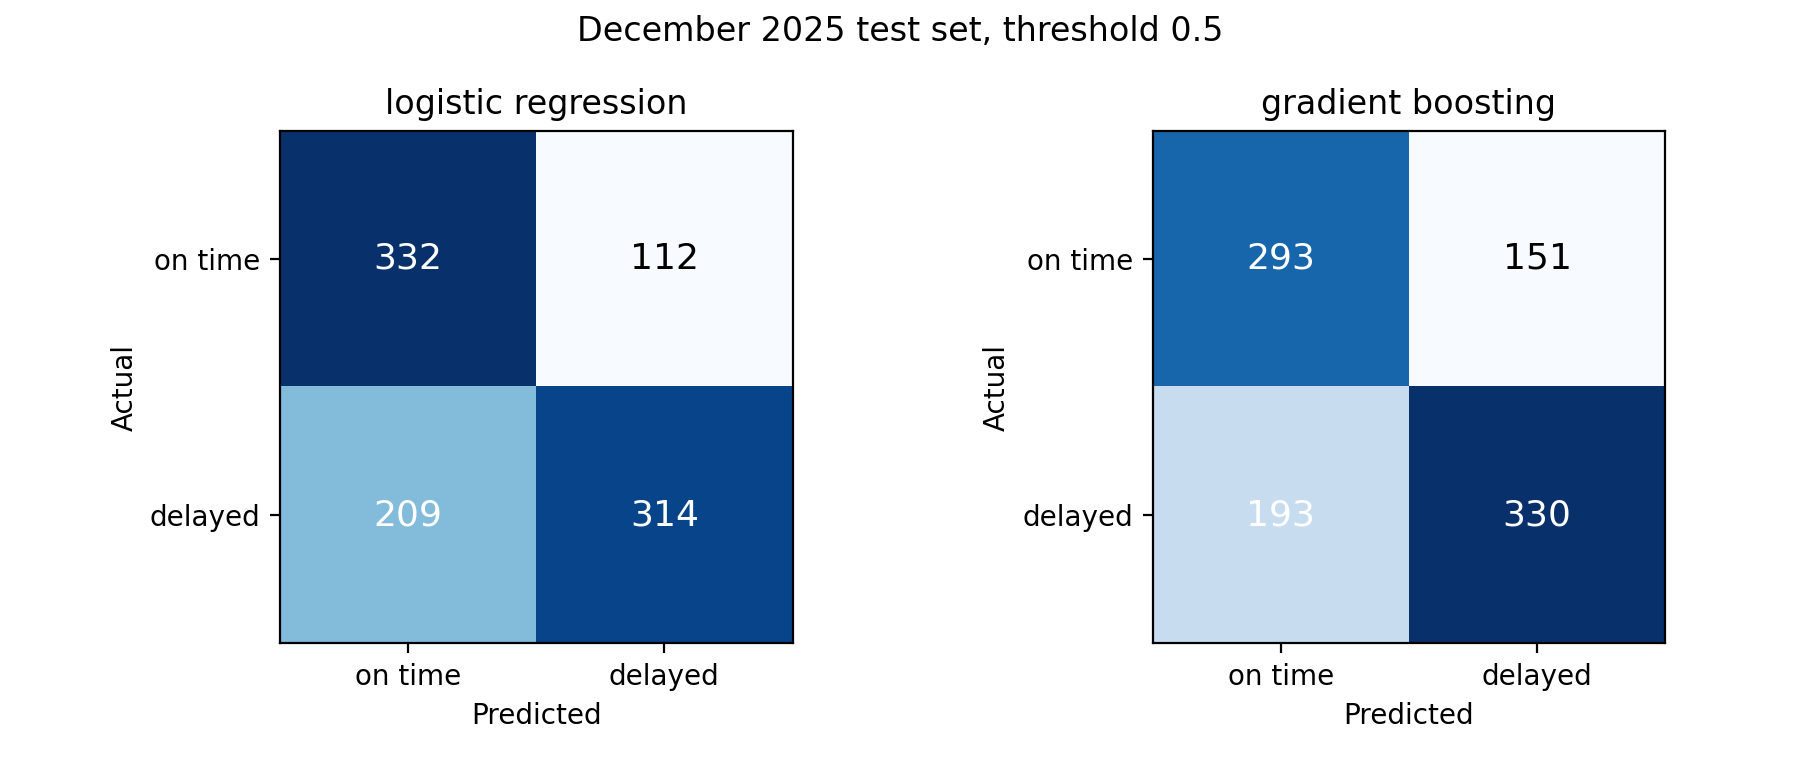
\includegraphics[width=\textwidth]{confusion_matrices_test}
  \caption{Confusion matrices of both models on the December test set at the threshold of 0.5. Rows show the actual class and columns the predicted class.}
  \label{fig:confusion}
\end{figure}

The models place their errors differently. The logistic regression is the more cautious model: it raises 112 false alarms, which is 25.2\% of the on-time flights, and it misses 209 delays, which is 40.0\% of the delayed flights. Gradient boosting flags more flights. It finds 16 more delayed flights than the logistic regression (330 compared with 314), and it pays for them with 39 additional false alarms (151 compared with 112). Its false alarm rate is 34.0\% and its miss rate is 36.9\%.

Both models predict fewer delays than occurred: they flag 44.1\% and 49.7\% of the flights, while the actual delayed share was 54.1\%. For both models the false negatives therefore outnumber the false alarms, by 209 against 112 for the logistic regression and by 193 against 151 for gradient boosting. This is consistent with models that were trained on months with a delayed share of 40.4\% and then met a month with a much higher share, and I examine it in the threshold analysis (\cref{sec:threshold}). For an operator, the practical reading is that a flagged flight is delayed in 74\% of the cases for the logistic regression and in 69\% for gradient boosting, while 40\% and 37\% of the delays occur without a warning.

\subsection{Precision-recall curves}\label{sec:pr}
\Cref{fig:pr} shows the precision-recall curves of both models on the December test set. The precision-recall view is useful here for a practical reason: it shows how many of the flights that a model flags are really delayed, and how many of the delayed flights it finds, over all possible thresholds and not only at 0.5. The dashed line is the no-skill level, which equals the delayed share of the test month, 54.1\%. The average precision, which summarizes each curve, is 0.784 for the logistic regression and 0.773 for gradient boosting. Both are clearly above the no-skill level, and the two curves are close to each other over most of the range.

\begin{figure}[ht]
  \centering
  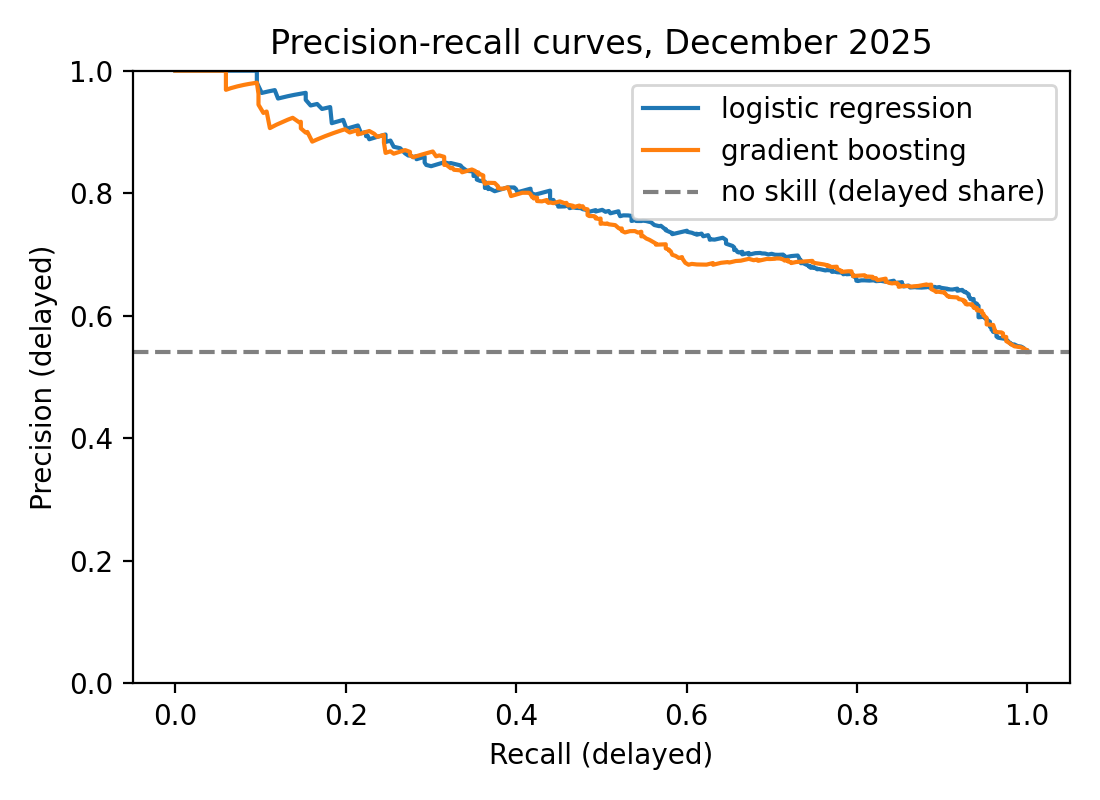
\includegraphics[width=0.7\textwidth]{precision_recall_test}
  \caption{Precision-recall curves of both models on the December test set. The dashed line marks the no-skill level of 54.1\%.}
  \label{fig:pr}
\end{figure}

The curves also show what a higher recall costs. At a recall of at least 50\%, the best attainable precision is 0.773 for the logistic regression and 0.751 for gradient boosting. At a recall of at least 70\% it falls to 0.700 and 0.694, and at a recall of at least 90\% to 0.645 and 0.639. A model that finds nearly all delayed flights therefore raises a false alarm for about one flag in three. Precision also depends on the delayed share of the period, which was unusually high in December. In a month with a lower delayed share, the same ranking would produce a lower precision, so I read these values as specific to the test month.

\subsection{Error analysis}\label{sec:errors}
I examined where the errors occur, using the saved tables of the notebook. For each group, I report the share of flights that the model flagged as delayed, the error rate, and the numbers of false positives (FP) and false negatives (FN). A false positive is an on-time flight that the model flagged as delayed, and a false negative is a delayed flight that it missed. The counts are not stored in the notebook tables. I derived them from the flagged share and the error rate of each group, and the sums over the groups match the confusion matrices in \cref{fig:confusion}.

\paragraph{By time of day.} \Cref{tab:error_time} groups the flights by the scheduled hour of arrival. The error rate is lowest at night, between 00 and 05, and in the afternoon and evening, at about 30\% to 38\%, and highest in the morning, between 06 and 11, at 43\% to 45\%. The two kinds of error differ clearly between the blocks. In the morning, both models flag few flights (12.0\% and 17.9\%), although about half of them are delayed, so almost all errors are false negatives. At night, the models flag 74.3\% and 85.6\% of the flights, above the 66.5\% that are delayed, and the false positives dominate. The afternoon block contains the largest group of 382 flights and the largest number of missed delays, 89 and 87. This pattern is consistent with a schedule-based score that rises through the day, but I cannot establish the cause from these data.

% tab_error_time.tex, source: results/error_by_time_of_day.csv of the analysis repository; the counts of false positives and
% false negatives are derived from the flagged share and the error rate of each group.
\begin{table}[ht]
  \centering
  \caption{Errors by scheduled hour of arrival on the December test set at the threshold of 0.5. FP is the number of false positives and FN the number of false negatives.}
  \label{tab:error_time}
  \begin{threeparttable}
    \footnotesize
    \setlength{\tabcolsep}{2pt}
    \begin{tabular*}{\textwidth}{@{\extracolsep{\fill}}lrrrrrrrrrr@{}}
      \toprule
      & & & \multicolumn{4}{c}{Logistic regression} & \multicolumn{4}{c}{Gradient boosting} \\
      \cmidrule(lr){4-7} \cmidrule(lr){8-11}
      Scheduled hour & Flights & Delayed (\%) & Flagged (\%) & Error (\%) & FP & FN & Flagged (\%) & Error (\%) & FP & FN \\
      \midrule
      00 to 05 & 167 & 66.5 & 74.3 & 30.5 & 32 & 19 & 85.6 & 29.9 & 41 & 9 \\
      06 to 11 & 117 & 49.6 & 12.0 & 42.7 & 3 & 47 & 17.9 & 45.3 & 8 & 45 \\
      12 to 17 & 382 & 53.1 & 38.5 & 31.9 & 33 & 89 & 41.4 & 33.8 & 42 & 87 \\
      18 to 23 & 301 & 50.2 & 46.8 & 32.6 & 44 & 54 & 52.8 & 37.2 & 60 & 52 \\
      \midrule
      All flights & 967 & 54.1 & 44.1 & 33.2 & 112 & 209 & 49.7 & 35.6 & 151 & 193 \\
      \bottomrule
    \end{tabular*}
    \begin{tablenotes}
      \footnotesize
      \item Delayed is the share of delayed flights in the group, flagged is the share that the model classified as delayed, and error is the share classified incorrectly.
    \end{tablenotes}
  \end{threeparttable}
\end{table}


\paragraph{By airline.} \Cref{tab:error_airline} shows the same analysis for each airline. Airlines are anonymized and ranked by the number of test flights, and all airlines with fewer than 30 test flights are pooled. Most groups are small, so their error rates are uncertain, and I do not rank the airlines by them. Two patterns stand out. For several airlines the models predict almost one class for every flight. Airlines 3 and 11 have delayed shares of 23.7\% and 22.6\%, and neither model flags any of their flights. Airline 5 has a delayed share of 11.1\%: the logistic regression flags none of its flights, while gradient boosting flags 31.1\%. At the other end, Airlines 4, 9, and 10 have delayed shares of 74.2\% to 83.8\%, and both models flag at least 95\% of their flights. This suggests that for these groups the models mainly follow the typical outcome of the airline in the fitting months, although I did not tabulate the delayed shares by airline for those months. The errors are then the flights that deviate from the predicted class. For Airlines 2 and 12, in contrast, the error rate of 43.5\% to 63.3\% is close to or above the level of a random guess, so the models have little information about these airlines.

% tab_error_airline.tex, source: results/error_by_airline.csv of the analysis repository; the counts of false positives and
% false negatives are derived from the flagged share and the error rate of each group.
\begin{table}[ht]
  \centering
  \caption{Errors by airline on the December test set at the threshold of 0.5. Airlines are anonymized and ranked by the number of test flights. FP is the number of false positives and FN the number of false negatives.}
  \label{tab:error_airline}
  \begin{threeparttable}
    \footnotesize
    \setlength{\tabcolsep}{2pt}
    \begin{tabular*}{\textwidth}{@{\extracolsep{\fill}}lrrrrrrrrrr@{}}
      \toprule
      & & & \multicolumn{4}{c}{Logistic regression} & \multicolumn{4}{c}{Gradient boosting} \\
      \cmidrule(lr){4-7} \cmidrule(lr){8-11}
      Airline & Flights & Delayed (\%) & Flagged (\%) & Error (\%) & FP & FN & Flagged (\%) & Error (\%) & FP & FN \\
      \midrule
      Other airlines & 230 & 50.9 & 30.0 & 41.7 & 24 & 72 & 37.0 & 42.6 & 33 & 65 \\
      Airline 1 & 219 & 65.8 & 58.0 & 33.3 & 28 & 45 & 59.8 & 35.2 & 32 & 45 \\
      Airline 2 & 85 & 49.4 & 12.9 & 43.5 & 3 & 34 & 8.2 & 48.2 & 3 & 38 \\
      Airline 3 & 76 & 23.7 & 0.0 & 23.7 & 0 & 18 & 0.0 & 23.7 & 0 & 18 \\
      Airline 4 & 68 & 79.4 & 100.0 & 20.6 & 14 & 0 & 95.6 & 22.1 & 13 & 2 \\
      Airline 5 & 45 & 11.1 & 0.0 & 11.1 & 0 & 5 & 31.1 & 28.9 & 11 & 2 \\
      Airline 6 & 40 & 42.5 & 20.0 & 37.5 & 3 & 12 & 45.0 & 47.5 & 10 & 9 \\
      Airline 7 & 38 & 55.3 & 81.6 & 47.4 & 14 & 4 & 100.0 & 44.7 & 17 & 0 \\
      Airline 8 & 37 & 78.4 & 78.4 & 16.2 & 3 & 3 & 78.4 & 16.2 & 3 & 3 \\
      Airline 9 & 37 & 83.8 & 97.3 & 18.9 & 6 & 1 & 100.0 & 16.2 & 6 & 0 \\
      Airline 10 & 31 & 74.2 & 96.8 & 22.6 & 7 & 0 & 100.0 & 25.8 & 8 & 0 \\
      Airline 11 & 31 & 22.6 & 0.0 & 22.6 & 0 & 7 & 0.0 & 22.6 & 0 & 7 \\
      Airline 12 & 30 & 50.0 & 56.7 & 60.0 & 10 & 8 & 86.7 & 63.3 & 15 & 4 \\
      \midrule
      All flights & 967 & 54.1 & 44.1 & 33.2 & 112 & 209 & 49.7 & 35.6 & 151 & 193 \\
      \bottomrule
    \end{tabular*}
    \begin{tablenotes}
      \footnotesize
      \item Other airlines pools all airlines with fewer than 30 test flights each. Delayed is the share of delayed flights in the group, flagged is the share that the model classified as delayed, and error is the share classified incorrectly.
    \end{tablenotes}
  \end{threeparttable}
\end{table}


Overall, the logistic regression makes fewer false positives (112 against 151) and gradient boosting makes fewer false negatives (193 against 209). Neither model is better in both respects, and which error matters more depends on operational costs that I do not have (\cref{sec:rule}).

\subsection{Threshold analysis}\label{sec:threshold}
\Cref{tab:threshold} shows how the macro F1 and the share of flagged flights change when the threshold moves between 0.30 and 0.70. This is a diagnosis on the test month and not a tuning step: the threshold in all other results stays at 0.5 (\cref{sec:rule}), and the values below must not be read as a recommendation.

% tab_threshold.tex, source: results/threshold_sensitivity.csv of the analysis repository.
\begin{table}[ht]
  \centering
  \caption{Macro F1 and share of flights flagged as delayed for different thresholds on the December test set. The actual delayed share is 54.1\%. The best macro F1 of each model is in bold, and the reported threshold is 0.50.}
  \label{tab:threshold}
  \begin{tabular*}{\textwidth}{@{\extracolsep{\fill}}lcccc@{}}
    \toprule
    & \multicolumn{2}{c}{Logistic regression} & \multicolumn{2}{c}{Gradient boosting} \\
    \cmidrule(lr){2-3} \cmidrule(lr){4-5}
    Threshold & Macro F1 & Flagged (\%) & Macro F1 & Flagged (\%) \\
    \midrule
    0.30 & 0.646 & 76.1 & 0.636 & 76.5 \\
    0.35 & 0.655 & 70.5 & 0.648 & 72.2 \\
    0.40 & 0.662 & 63.5 & 0.667 & 62.9 \\
    \textbf{0.45} & \textbf{0.680} & \textbf{56.6} & \textbf{0.669} & \textbf{56.0} \\
    0.50 & 0.668 & 44.1 & 0.644 & 49.7 \\
    0.55 & 0.648 & 36.0 & 0.643 & 39.0 \\
    0.60 & 0.628 & 29.7 & 0.621 & 30.2 \\
    0.65 & 0.593 & 24.0 & 0.576 & 21.1 \\
    0.70 & 0.558 & 18.4 & 0.528 & 15.4 \\
    \bottomrule
  \end{tabular*}
\end{table}


Two findings stand out. First, the macro F1 is fairly flat in the middle of the range. Between 0.35 and 0.55, it stays between 0.648 and 0.680 for the logistic regression and between 0.643 and 0.669 for gradient boosting. Outside this range it drops, to 0.558 and 0.528 at a threshold of 0.70, because the models then flag only 18.4\% and 15.4\% of the flights. Second, the best value for both models is at 0.45, where the macro F1 is 0.680 for the logistic regression and 0.669 for gradient boosting. This is higher than at 0.5 by 0.012 and 0.025. At 0.45, the models flag 56.6\% and 56.0\% of the flights, which is close to the actual delayed share of 54.1\%. The threshold of 0.5 flags fewer flights (44.1\% and 49.7\%), and this agrees with the observation in \cref{sec:confusion} that the models predict fewer delays than occurred.

The result has two limits. The gain from 0.45 is small compared with the width of the bootstrap intervals in \cref{tab:metrics}, so I cannot say that 0.45 is better than 0.5 in general. The best threshold would also differ in a month with another delayed share, because the models were trained on months in which about 40\% of the flights were delayed. For operational use, the threshold should therefore be set on the basis of the cost of a false alarm compared with a missed delay, which I do not have. The table helps to make this choice, because it shows the share of flights that an operator would have to handle at each threshold.

\subsection{Robustness analysis}\label{sec:robustness}
The ledger contains rows that could distort the results (\cref{sec:data}). I tested whether they matter by repeating the final fit and the test evaluation after removing them. \Cref{tab:robustness} shows the result for three variants. The first is the reported analysis. The second removes the 26 flights with the remark \col{TEST}, all of which fall into the fitting months. The third also removes the 118 rescheduled flights, of which 109 are in the fitting months and 9 in the test month. The selected settings were kept, and the models were not tuned again.

% tab_robustness.tex, source: results/robustness_row_exclusions.csv of the analysis repository.
\begin{table}[ht]
  \centering
  \caption{Test results after the exclusion of unusual rows. Each variant refits both models on the remaining January to November flights with the selected settings and scores them on the remaining December flights at the threshold of 0.5.}
  \label{tab:robustness}
  \footnotesize
  \setlength{\tabcolsep}{4pt}
  \begin{tabular}{@{}>{\raggedright\arraybackslash}p{4.4cm}rrcccc@{}}
    \toprule
    & & & \multicolumn{2}{c}{Logistic regression} & \multicolumn{2}{c}{Gradient boosting} \\
    \cmidrule(lr){4-5} \cmidrule(lr){6-7}
    Variant & Fit rows & Test rows & Macro F1 & ROC AUC & Macro F1 & ROC AUC \\
    \midrule
    All rows (reported results) & \num{9896} & 967 & 0.668 & 0.749 & 0.644 & 0.739 \\
    Without remark \col{TEST} & \num{9870} & 967 & 0.669 & 0.749 & 0.646 & 0.742 \\
    Without \col{TEST} and rescheduled & \num{9761} & 958 & 0.668 & 0.748 & 0.653 & 0.743 \\
    \bottomrule
  \end{tabular}
\end{table}


The results are stable. The macro F1 of the logistic regression changes by at most 0.001, from 0.668 to 0.669 and back, and its ROC AUC by at most 0.001. For gradient boosting, the macro F1 rises from 0.644 to 0.646 and then to 0.653, and its ROC AUC from 0.739 to 0.743. The largest change is therefore 0.009 for the macro F1 and 0.004 for the ROC AUC, which is much smaller than the bootstrap intervals in \cref{tab:metrics}. In all three variants, the logistic regression is ahead of gradient boosting in both metrics, but the gap in macro F1 shrinks from 0.024 to 0.015. I take this as a sign that the two models are close, and not as a change in the conclusion. I did not test other exclusions, for example of the early arrivals or of the duplicated rows, because they affect only three and eight flights.

% 07_limitations.tex: Section 6.
\section{Limitations}\label{sec:limitations}

The results in this report support a limited conclusion, and I list here the reasons for this limit. I order them by how strongly they affect the interpretation of the results.

\paragraph{One test month.} All test results come from December 2025, which contains 967 flights. The bootstrap intervals in \cref{tab:metrics} show that the metrics vary with the choice of test days, and a different month would give different values. The test month is also not typical: its delayed share of 54.1\% is much higher than the 40.9\% of the training months and the 35.5\% of the validation month. Both models flagged fewer delays than occurred (\cref{sec:confusion}), and the accuracy of the majority baseline depends on the delayed share as well. I therefore treat the absolute values of accuracy, precision, and recall as specific to December, and I give more weight to the ROC AUC, which does not depend on the delayed share.

\paragraph{Fixed threshold.} I used the threshold of 0.5 for all reported results (\cref{sec:rule}). The threshold analysis shows that another threshold would give a different balance of false alarms and missed delays (\cref{sec:threshold}). I did not choose a threshold from the costs of the two errors, because I do not have this information, and a threshold chosen on the test month would not be a fair estimate of the performance on new data.

\paragraph{Schedule-only features.} The models use seven variables that are part of the schedule (\cref{sec:features}). I excluded all information that becomes known at or after arrival, which is necessary for a valid prediction, but it also means that the models cannot see the causes of delays that an operator can observe, such as weather, the delay of the inbound flight, or the situation on the apron. The moderate ROC AUC of 0.74 to 0.75 is therefore not surprising. It shows how much the schedule alone says about the delay, and it is not an upper limit for what a better-informed system could reach.

\paragraph{Rescheduled flights.} The ledger contains 118 flights whose remark marks them as rescheduled, and for these flights, STA may not describe the plan that the airline actually followed. The target is the difference to the recorded STA, so the delay of such a flight may be overstated or understated, and I cannot verify this from the data. I kept these flights in the main analysis and tested their removal in \cref{sec:robustness}. The results changed little, but the test only covers the flights that carry the remark, and other changes of the plan may not be marked.

\paragraph{Scope of the uncertainty estimates.} The bootstrap resamples the 31 test days, and the models are not refitted (\cref{sec:bootstrap}). The intervals therefore measure how the metrics depend on the test days. They do not measure the uncertainty from the training data, from the selection of the settings on a single validation month of 902 flights, or from the seed. The comparison of the two models is also limited: the settings of both were selected within a range of about 0.01 macro F1 on the validation month, and the paired difference on the test month is small. I do not claim that one model is better in general. In addition, the bootstrap, the threshold analysis, and the robustness analysis reuse the December data as a diagnosis, although none of them changed a setting.

\paragraph{Small groups.} The error analysis in \cref{sec:errors} rests on small groups. Most airlines have fewer than 100 test flights, and the pooled group of smaller airlines mixes operators with different behavior. I did not compute intervals for these groups, and their error rates should be read as descriptions of the test month and not as properties of the airlines. The counts of false positives and false negatives are derived from the saved tables and not taken from the notebook directly.

\paragraph{Probabilities.} Both models use balanced class weights, so their scores are not calibrated probabilities (\cref{sec:models}). I used them only to rank flights and to apply a threshold. I did not evaluate calibration, and the scores should not be interpreted as the chance of a delay.

\paragraph{Non-public data.} The ledger is restricted and cannot be shared (\cref{sec:data}). Other researchers can inspect the code and the aggregated results in the repository, but they cannot rerun the analysis without the ledger, which is held by AIBD LAS and would need to be requested from AIBD LAS. Airline names are anonymized in the saved tables, so the airline-level results cannot be matched to real operators outside the project.

\paragraph{Generalizability.} The data cover one airport and one calendar year. The models learned the patterns of AIBD in 2025, such as the typical delay of an airline at a given hour, and these patterns can change with a new schedule, new airlines, or new operating conditions. A level of performance like the one in this report should not be expected at another airport or in another year without a new evaluation. Because the training months come before the test month, the setup does reflect the use of a model on future flights at AIBD, but I tested it for one month only.

% 08_conclusion.tex: Section 7.
\section{Conclusion}\label{sec:conclusion}

I asked whether the delay of an arrival at AIBD, defined as \blockon{} later than STA by more than 15 minutes, can be predicted from information that is known before the aircraft arrives. For this purpose, I built a chronological evaluation on the 2025 ledger of \num{10863} flights, restricted the models to seven schedule variables, and tested them on the last month of the year.

The main finding is that the schedule carries some, but limited, information about delays. On the December test set, the logistic regression reaches a macro F1 of 0.668 and a ROC AUC of 0.749, and gradient boosting reaches 0.644 and 0.739. Both models are clearly better than the majority baseline, which has a macro F1 of 0.315, and both are clearly above the no-skill level in the precision-recall analysis. The logistic regression is ahead of gradient boosting in all three robustness variants, but the difference is small (0.024 macro F1, with an interval from 0.005 to 0.042), and the two models were practically tied on the validation month. I therefore do not conclude that the more flexible model has an advantage on these data.

The error analysis and the threshold analysis show where the models are weak. They miss many delays in the morning and for several airlines, and at the threshold of 0.5 they flag fewer flights than were delayed in December. Moving the threshold to 0.45 improves the macro F1 of both models in this month, but I report it only as a diagnosis, and a threshold for operational use would need the costs of the two kinds of error.

What the results support is a first screening tool: a model of this kind could rank the scheduled arrivals of the next days by their risk of delay, so that planners can look at the flights with the highest scores first. What they do not support is a reliable warning for single flights, because 37\% to 40\% of the delays occurred without a flag, and because the evidence comes from one test month at one airport (\cref{sec:limitations}).

Three steps would strengthen the evidence. The first is a rolling evaluation over several test months, so that the variation between months is measured and not only the variation between days. The second is to add information that is available before arrival, for example the status of the inbound flight and the weather forecast, which would address the main limit of a schedule-only model. The third is to choose the threshold from the operational costs of false alarms and missed delays, and to check the calibration of the scores before they are used for decisions.


% Statement on the use of AI tools: unnumbered, just before the references.
% 09_ai_statement.tex: statement on the use of AI tools (unnumbered, placed before the references).
% DRAFT: rewrite this statement in your own words before submitting. Every sentence must be true.
\section*{Statement on the Use of AI Tools}

I used one AI tool in this project, the assistant Claude (Anthropic). I describe here what the tool did, what I did, and where the wording of this report comes from.

\paragraph{Notebook.} Claude drafted parts of the notebook code, and I wrote the other parts myself. I ran the code, checked the outputs, and adapted the code where it was needed. I also used Claude to find errors in the code and to have design options explained to me.

\paragraph{Report.} Claude drafted the text of this report, section by section, on the basis of my notebook, my saved result tables, and my README, and it typeset the tables and the document in LaTeX. I read each section, asked for changes, and accepted the final version, so most of the wording comes from the suggestions of the tool. Claude also checked the numbers in the report against my result files, and it computed a small number of values from my saved files: the counts of false positives and false negatives in \cref{tab:error_time,tab:error_airline}, which the text describes as derived, and the precision at fixed levels of recall in \cref{sec:pr}. Some readings of the results, for example the use as a first screening tool and the next steps in \cref{sec:conclusion}, were proposed by the tool, and I kept them because I agree with them.

\paragraph{My own contribution.} The topic and the data are mine. I made the decisions of the analysis: the chronological split, the fixed threshold of 0.5, and the treatment of the unusual rows.

\paragraph{Responsibility.} I treated the outputs of the tool as suggestions and not as authoritative sources. I checked the code and the content that I adopted, and I take responsibility for the report, the code, and the results.


% References: only entries that are cited in the text are printed.
\bibliography{references}

% Appendices: lettered A, B, ...
\appendix
% A_reproducibility.tex: Appendix A.
\section{Reproducibility}\label{app:reproducibility}

This appendix lists what is needed to repeat the analysis. The complete pipeline is one Jupyter notebook, which runs from the loading of the ledger to the saved result tables and figures.

\paragraph{Software and seed.} The analysis ran with Python 3.12.12, pandas 2.3.3, NumPy 2.3.5, scikit-learn 1.7.2, and Matplotlib 3.10.6, as listed in \cref{tab:software}. The versions are pinned in the file \col{requirements.txt}, together with JupyterLab (version 4 or later), and they are also written to \col{results/run_info.txt} at the end of each run. The random seed is 42. It is used in the models and in the bootstrap.

\paragraph{Repository.} The code and the saved outputs are available at \url{https://github.com/mohameth-gueye/aibd-arrival-delay-retake}. The repository contains the notebook with its saved outputs, the folder \col{results/} with the aggregated tables (metrics, confidence intervals, error analysis, threshold sensitivity, and robustness) and the run information, the folder \col{figures/} with the confusion matrices and the precision-recall curves, and the requirements file. The folder \col{data/} is not tracked, because the ledger is restricted. Airline names are anonymized in all saved tables.

\paragraph{Steps to rerun the notebook.} The following steps repeat the analysis, if the ledger is available.
\begin{enumerate}[label=\arabic*.,leftmargin=*,itemsep=2pt]
  \item Request the ledger from AIBD LAS (see below). Save the file in the project folder as \col{data/aibd_2025_regular_arrivals.csv} and keep it out of version control.
  \item Create and activate a virtual environment with Python 3.12, and install the packages with \col{pip install -r requirements.txt}.
  \item Start JupyterLab from the project root, because the notebook uses the relative paths \col{data/}, \col{results/}, and \col{figures/}.
  \item Open the notebook and choose Restart and Run All. The run rebuilds all tables and figures in this report, and the values should agree with it for the same package versions.
\end{enumerate}

\paragraph{Data access.} The ledger is held by AIBD LAS \citep{aibd2025ledger}. It is not public, and access would need to be requested from AIBD LAS. Without the data, the saved outputs in the notebook and in \col{results/} show what the analysis produced, but the pipeline cannot be rerun, and row-level predictions are not shared.

\FloatBarrier
% B_validation.tex: Appendix B.
\section{Validation Results}\label{app:validation}

This appendix documents the model selection of \cref{sec:tuning}. All numbers come from the November validation month, on which the settings were chosen. They are not test results and should not be compared with \cref{tab:metrics}, because the delayed share of November (35.5\%) differs strongly from that of December (54.1\%).

\Cref{tab:val_metrics} shows the metrics of the three models with the selected settings. The two trained models beat the majority baseline, which reaches an accuracy of 0.645 but a macro F1 of only 0.392. Logistic regression and gradient boosting are practically tied, with macro F1 values of 0.649 and 0.651 and ROC AUC values of 0.699 and 0.700. At the threshold of 0.5, the logistic regression flags 378 of the 902 flights, of which 199 are delayed, and it misses 121 of the 320 delayed flights. Gradient boosting flags 393 flights, of which 206 are delayed, and it misses 114 delayed flights.

% tab_val_metrics.tex, source: notebook section 15 (Validation comparison).
\begin{table}[H]
  \centering
  \caption{Metrics on the November validation month (902 flights, 35.5\% delayed) at the threshold of 0.5. The models were fitted on January to October with the selected settings.}
  \label{tab:val_metrics}
  \footnotesize
  \setlength{\tabcolsep}{3pt}
  \begin{tabular*}{\textwidth}{@{\extracolsep{\fill}}lccccccc@{}}
    \toprule
    Model & Accuracy & Macro F1 & F1 (delayed) & Precision & Recall & ROC AUC & PR AUC \\
    \midrule
    Majority class & 0.645 & 0.392 & 0.000 & 0.000 & 0.000 & 0.500 & 0.355 \\
    Logistic regression & 0.667 & 0.649 & 0.570 & 0.526 & 0.622 & 0.699 & 0.582 \\
    Gradient boosting & 0.666 & 0.651 & 0.578 & 0.524 & 0.644 & 0.700 & 0.586 \\
    \bottomrule
  \end{tabular*}
  \par\smallskip
  {\footnotesize Precision and recall refer to the delayed class. PR AUC is the average precision, and the no-skill value equals the delayed share of 0.355.\par}
\end{table}


\Cref{tab:val_grid_lr,tab:val_grid_gb} list the eight best settings of each model. The selected settings are the first rows: $C=0.3$ with a minimum frequency of 10 for the logistic regression, and a learning rate of 0.05, 8 leaves, a leaf size of 60, 100 trees, and a minimum frequency of 60 for gradient boosting. The macro F1 of the eight best settings lies between 0.640 and 0.649 for the logistic regression and between 0.641 and 0.651 for gradient boosting. The first-ranked setting leads the second by only 0.004 and 0.005, and several settings share the same macro F1 and differ in the third decimal of the ROC AUC. The selection among these settings is therefore not sharp. Seven of the eight best gradient boosting settings use 100 trees, and six use 8 leaves, which is consistent with a model that profits from strong limits on its complexity.

% tab_val_grid_lr.tex, source: notebook section 13 (Logistic regression tuning).
\begin{table}[H]
  \centering
  \caption{The eight best of the 15 logistic regression settings on the validation month, ranked by macro F1 and, for ties, by ROC AUC. The selected setting is in bold.}
  \label{tab:val_grid_lr}
  \footnotesize
  \begin{tabular*}{0.8\textwidth}{@{\extracolsep{\fill}}cccccc@{}}
    \toprule
    Rank & $C$ & Min.\ frequency & Macro F1 & ROC AUC & PR AUC \\
    \midrule
    \textbf{1} & \textbf{0.3} & \textbf{10} & \textbf{0.649} & \textbf{0.699} & \textbf{0.582} \\
    2 & 0.1 & 10 & 0.645 & 0.698 & 0.584 \\
    3 & 0.1 & 30 & 0.645 & 0.698 & 0.588 \\
    4 & 1.0 & 60 & 0.645 & 0.698 & 0.586 \\
    5 & 0.3 & 30 & 0.643 & 0.698 & 0.588 \\
    6 & 1.0 & 10 & 0.642 & 0.696 & 0.574 \\
    7 & 0.1 & 60 & 0.642 & 0.699 & 0.582 \\
    8 & 0.3 & 60 & 0.640 & 0.699 & 0.585 \\
    \bottomrule
  \end{tabular*}
\end{table}


% tab_val_grid_gb.tex, source: notebook section 14 (Gradient boosting tuning).
\begin{table}[H]
  \centering
  \caption{The eight best of the 48 gradient boosting settings on the validation month, ranked by macro F1 and, for ties, by ROC AUC. The selected setting is in bold. Rate is the learning rate, min.\ freq.\ the minimum frequency for pooling rare categories, leaves the maximum number of leaf nodes, leaf size the minimum number of flights per leaf, and trees the number of boosting iterations.}
  \label{tab:val_grid_gb}
  \footnotesize
  \setlength{\tabcolsep}{3pt}
  \begin{tabular*}{\textwidth}{@{\extracolsep{\fill}}ccccccccc@{}}
    \toprule
    Rank & Rate & Leaves & Leaf size & Trees & Min.\ freq. & Macro F1 & ROC AUC & PR AUC \\
    \midrule
    \textbf{1} & \textbf{0.05} & \textbf{8} & \textbf{60} & \textbf{100} & \textbf{60} & \textbf{0.651} & \textbf{0.700} & \textbf{0.586} \\
    2 & 0.05 & 8 & 20 & 100 & 60 & 0.646 & 0.699 & 0.584 \\
    3 & 0.10 & 8 & 20 & 100 & 60 & 0.644 & 0.700 & 0.585 \\
    4 & 0.10 & 8 & 60 & 100 & 60 & 0.643 & 0.701 & 0.591 \\
    5 & 0.10 & 16 & 60 & 100 & 10 & 0.643 & 0.698 & 0.580 \\
    6 & 0.05 & 8 & 60 & 300 & 60 & 0.642 & 0.697 & 0.588 \\
    7 & 0.05 & 16 & 60 & 100 & 60 & 0.642 & 0.703 & 0.587 \\
    8 & 0.10 & 8 & 20 & 100 & 10 & 0.641 & 0.694 & 0.574 \\
    \bottomrule
  \end{tabular*}
\end{table}



\end{document}
